\iffabian
	\subsection{Launcher}
	\label{sec:win-launcher}
\else
	\section{Launcher}
	\label{sec:win-launcher}
\fi
Der Launcher ist ein eigenes Fenster, welches vor dem Öffnen der Benutzeroberfläche angezeigt wird. Hier hat der Benutzer die Möglichkeit, eigene Profile zu erstellen, die Sprache zu ändern und sein Benutzerprofil zu starten. Auch werden hier die zuletzt geöffneten Profile dargestellt.

\begin{figure}[h] 
  \centering
     \includegraphics[width=0.9\textwidth]{./media/images/gui/launcher/launcher_main.png}
  \caption{Launcher GUI}
  \label{fig:launcher_GUI}
\end{figure}

%TODO Verwei auf Anhang
Grundsätzlich ist der Launcher ein JFrame\footnote{\url{http://www.java-tutorial.org/jframe.html}}, das vor dem Start der Benutzeroberfläche angezeigt wird. Die zuletzt verwendeten Profile werden mithilfe einer JScrollpane\footnote{\url{http://www.java2s.com/Tutorial/Java/0240__Swing/CreatingaJTable.htm}}  in welcher mehrere JPanels\footnote{\url{https://docs.oracle.com/javase/tutorial/uiswing/components/panel.html}} liegen, angezeigt. In den JPanels befinden sich der Name und das Benutzerbild.

\begin{itemize}
\item Falls in der Liste, kein Profil vorhanden ist, wird auf die Erstellung eines neuen Profils hingewiesen.
\item Wenn der Benutzer kein Profilbild gewählt hat, wird ein voreingestelltes Profilbild verwendet.
\item Mit einem Klick auf das Profilbild kann das gewünschte Profil geöffnet werden.
\item Es besteht die Möglichkeit, C Compact mithilfe des Launchers ohne Profil zu starten. Das bedeutet, dass kein Profil ausgewählt wurde und die Entwicklungsumgebung ohne Quest-System geöffnet wird.
\end{itemize}

\iffabian
	\subsubsection*{Erstellen eines neuen Profils}
\else
	\subsection{Erstellen eines neuen Profils}
\fi
Durch einen Klick auf den Button "`\textit{Neu}"' wird ein Fenster geöffnet, in dem man sein Profil erstellen kann.  

%TODO Anhang Referenzieren
Zuerst wird der Ordnerpfad mithilfe eines JFileChoosers (siehe Kapitel \ref{sec:JFileChooser}) abgefragt. Unter Verwendung einer JOptionPane\footnote{\url{http://docs.oracle.com/javase/7/docs/api/javax/swing/JOptionPane.html}}  (Abbildung: \ref{fig:JOptionPane}) kann nun der gewünschte Nutzername gewählt werden.
\begin{figure}[h] 
   \centering
     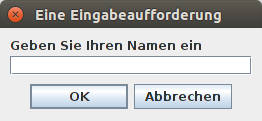
\includegraphics[width=0.3\textwidth]{./media/images/gui/launcher/JOptionPane.png}
  \caption{JOptionPane}
  \label{fig:JOptionPane}
\end{figure}

\begin{lstlisting}[language=JAVA]
String name = JOptionPane.showInputDialog(null,
"Bitte Namen eingeben:",
 " Eingabeaufforderung",JOptionPane.PLAIN_MESSAGE);
p.setName(name);
\end{lstlisting}

Wenn die Eingabe erfolgreich war, wird nun im gewählten Pfad ein neuer Ordner erstellt, welcher das Profil mit dem gewählten Namen repräsentiert. Darin befindet sich eine "`\textit{\textbf{profile.cp}}"' Datei, diese beinhaltet die Benutzereinstellungen. Sobald alle Eingaben getätigt wurden, wird die Entwicklungsumgebung mit dem neu gestalteten Profil gestartet.

Tritt bei der Erstellung eines Profils ein Fehler auf, zeigt eine JOptionpane die zugehörige Fehlermeldung an. Danach öffnet sich automatisch wieder der Lauchner. 

\iffabian
	\subsubsection*{Finden eines bereits existierenden Profils}
\else
	\subsection{Finden eines bereits existierenden Profils}
\fi
Damit ein Profil geöffnet werden kann, welches nicht in der Liste der Profile im Launcher vorhanden ist, muss eine Funktion vorhanden sein, mit welcher Profile gefunden werden kann.

Sobald man auf den Button "`\textbf{Finden}"' klickt, wird ein veränderter JFileChooser geöffnet. Hier kann nur eine "`\textit{\textbf{.cp}}"' Datei ausgewählt werden. Sobald diese angeklickt wird, werden das Profilbild und der Profilname als Vorschau auf der rechten Seite angezeigt. Wenn der Nutzer kein Profilbild eingestellt hat, wird hier ein voreingestelltes Profilbild angezeigt.

\begin{figure}[h] 
   \centering
     \includegraphics[width=0.9\textwidth]{./media/images/gui/launcher/launcher_finden.png}
  \caption{ Profilvorschau}
  \label{fig:Bild1}
\end{figure}

Indem man auf den "`\textbf{Öffnen}"'-Button klickt, startet man nun C-Compact mit dem gerade ausgewählten Profil und es wird zu den zuletzt verwendeten Profilen hinzugefügt.
